\section{Gestión de la información}

  \paragraph{}Para todas y cada una de las zonas de las que se compone esta
  aplicación (Administrador principal, Administrador de centro, Asesor y
  Alumno), la interfaz compartirá bastantes detalles en común, diferenciándose
  cada una de ellas del resto en el contenido que puede ver y gestionar el
  usuario que está ejecutando la aplicación, teniendo en cuenta el rol con el
  que participa. Por ejemplo, un usuario asesor no podrá ver determinadas zonas
  para la creación de una nueva titulación, ya que es una tarea que no le
  concierne.

  \paragraph{}Teniendo en cuenta lo anterior, a continuación se muestra una
  captura de pantalla para ejemplificar el diseño de la interfaz común a todas
  las zonas de la aplicación. Se ha utilizado la zona del Administrador
  principal por ser la más completa; pero, como se ha comentado antes, el resto
  de zonas comparten los mismos criterios de diseño, por lo cual la
  navegabilidad y usabilidad no varía entre zonas. La figura
  \ref{capturaGestionInformacion} muestra un ejemplo del diseño de la interfaz
  común.

  \begin{figure}[!ht]
    \begin{center}
      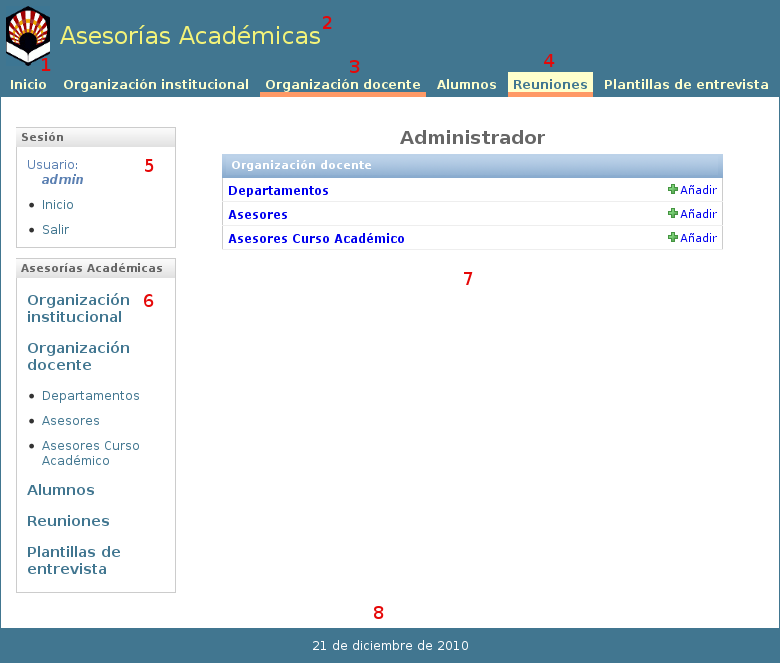
\includegraphics[scale=0.6]{12.Disenyo_Interfaz/12.3.Gestion_Informacion/gestion_informacion.png}
      \caption{Captura de pantalla de la gestión de la información.}
      \label{capturaGestionInformacion}
    \end{center}
  \end{figure}


  \paragraph{}Los elementos de la interfaz a destacar están señalados en la
  imagen con números rojos. A continuación se pasan a detallar:

  \begin{enumerate}
    \item \textbf{Logotipo de la Universidad de Córdoba}. Se trata de un
    enlace que, al pinchar sobre él, nos lleva directamente a la página
    principal de la Universidad de Córdoba (\url{http://www.uco.es}).
    \item \textbf{Nombre completo de la aplicación}.
    \item \textbf{Sección activa}. Se trata de la sección de la aplicación donde
    se encuentra el usuario en un momento determinado.
    \item \textbf{Ir a sección}. Se activa cuando el cursor del ratón se
    encuentra encima del enlace a una determinada sección. Si pulsamos el botón
    del ratón navegaremos hasta la sección indicada.
    \item \textbf{Menú de sesión}. Este menú contiene detalles acerca de la
    sesión que se encuentra ejecutando en un momento determinado.
    \begin{itemize}
      \item Para todas las zonas de la aplicación (Administrador principal,
      Administrador de centro, Asesor y Alumno) estará visible el nombre de
      usuario que ha iniciado la sesión, así como un enlace directo para ir al
      inicio de cada zona, y un enlace para salir de la sesión, el cual
      desconecta al usuario del sistema.
      \item Para la zona del administrador de centro se mostrará, además,
      el centro que sea objeto de administración en ese momento.
      \item Para las zonas de Asesor y Alumno se mostrará, además, el curso
      académico que sea objeto de administración en ese momento.
    \end{itemize}

    \item \textbf{Menú de secciones}. Es un menú de accesos rápidos para las
    distintas opciones de las que se compone la sección en la que se encuentra
    el usuario en un determinado momento, así como accesos al resto de
    secciones de la aplicación.
    \item \textbf{Contenido}. En la zona de contenido se mostrará la distinta
    información que sea necesario detallar en cada momento, teniendo en cuenta
    dónde se encuentre el usuario en un determinado momento.
    \item \textbf{Pie de página}. Zona utilizada para exponer alguna otra
    información que se quiera reflejar. Para esta aplicación se ha utilizado
    la fecha actual como información en el pie de página.
  \end{enumerate}
